\section{Predictions in ongoing actions}
\label{sec:prediction}

A critical aspect of video models regardless of the downstream task has been their ability to capture temporal information \citep{huang2018makes}. Learning temporal patterns can enable models to predict what is currently happening in a video, without having seen the full action or activity. We start by defining methods that aim to provide semantic predictions on the action categories from partial observations in \Cref{sec:prediction::EAP}. We then discuss approaches that generate unobserved frames in \Cref{sec:prediction::VFP}. States of actions or objects can change at different times during the execution of an action. We explore groups of tasks that predict the states of objects and actions in \Cref{sec:prediction::states}. 

\begin{figure}[t]
    \centering
    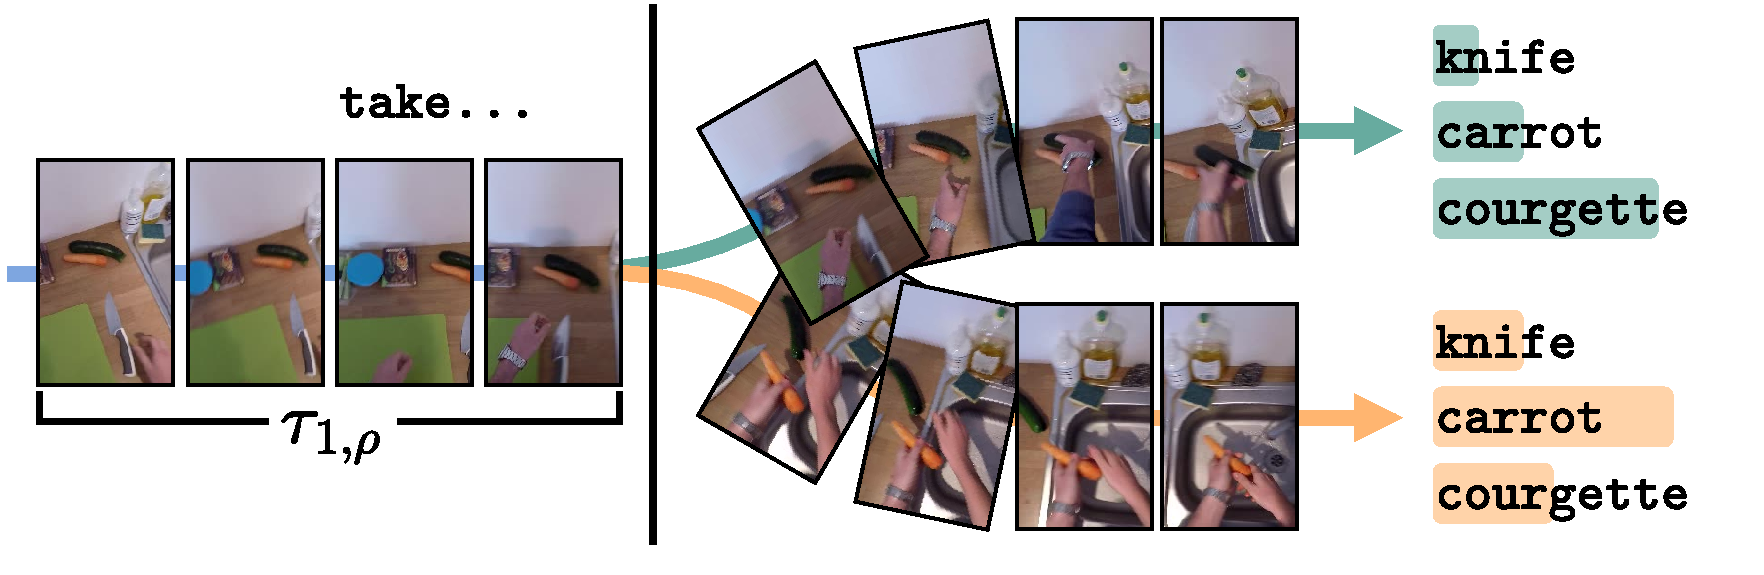
\includegraphics[width=\linewidth]{figs/EAP.pdf}
    \caption{\textbf{Early Action Prediction (EAP)}. Only the observable part of a video $\tau_{1,\rho}$ is used to predict the current action. EAP is challenging as the immediate future is often unpredictable especially when distinguishing between fine-grained actions, e.g., \textit{taking courgette} or \textit{taking carrot}. Video from \citet{damen2022rescaling}.}
    \label{fig:EAP_overview}
\end{figure}


\subsection{Early action prediction}
\label{sec:prediction::EAP}

Early Action Prediction (EAP) assumes an \emph{ongoing} action is being performed with predictions made based on the observable part of the action $\tau_{1,\rho}$ as shown in \Cref{fig:EAP_overview}. %Understanding actions from partial observations is a core capability of human cognition that relies on associating the sequentiality of temporal patterns to high-level semantics.
Several different lines of research have been explored to address relationships between partial action observation and high-level semantics.

\subsubsection{Challenges}

One of the main challenges that arise from partially observed videos is the \textbf{procedural proximity} in the execution of actions. As shown in \Cref{fig:EAP_overview}, there can be an overlap in the steps taken to perform similar activities. For the example shown, the difference between \textit{take courgette} and \textit{take carrot} is subtle, without significant motion variations. Instead, the distinction only becomes visually apparent at the end of the action. This challenge relates to the more general problem of \textbf{abstracted views} in which deterministic information relevant to the task is not always available. Although such fine-grained predictions may not be available, it is still possible to identify general categories for the actions being performed, e.g., \textit{take} $<$object$>$. An \textbf{adjustability requirement} is thus introduced as part of EAP to address the intrinsic uncertainty in partial observation.


\begin{figure}[t]
    \centering
    \begin{overpic}[width=\linewidth]{figs/EAP_clusters_ul.pdf}
    % Probabilistic modeling
    \put (36,23.9) {1.}
    \put (25.5,25.8) {2.}
    \put (22,20.2) {3.}
    \put (34.5,19) {4.}
    \put (37.5,29) {5.}
    \put (40.5,23) {6.}
    \put (51,27) {7.}
    % Temporal ordering
    \put (8,14) {8.}
    \put (14,11) {9.}
    \put (42.5,17.7) {10.}
    \put (42.5,8.5) {11.}
    \put (38,13.5) {12.}
    \put (23,12.5) {13.}
    \put (30,8.8) {14.}
    \put (20.5,7.7) {15.}
    \put (37.5,11) {16.}
    \put (53,10.8) {17.}
    \put (31.5,12.4) {18.}
    % Knowledge Distillation
    \put (74,18.8) {19.}
    \put (75.4,11.5) {20.}
    \put (81,18) {21.}
    \put (64,16.5) {22.}
    \put (59,25) {23.}
    \put (65.5,27.8) {24.}
    \put (88.5,19) {25.}
    \put (87.5,26.7) {26.}
    \put (55.4,18.5) {27.}
    \end{overpic}
    \resizebox{\linewidth}{!}{
    \begin{tabular}{lll}
         1. \citet{cao2013recognize} &
         2. \citet{hoai2014max} & 
         3. \citet{li2012modeling} \\
         4. \citet{li2014prediction} &
         5. \citet{ryoo2011human} &
         6. \citet{suris2021learning} \\
         7. \citet{chen2022ambiguousness} &
         8. \citet{misra2016shuffle} &
         9. \citet{zhou2015temporal} \\
         10. \citet{xu2015activity} &
         11. \citet{kong2014discriminative} &
         12. \citet{kong2018action} \\
         13. \citet{zhao2019spatiotemporal} &
         14. \citet{wu2021spatial} &
         15. \citet{wu2021anticipating} \\
         16. \citet{wang2023magi} &
         17. \citet{stergiou2023wisdom} &
         18. \citet{rangrej2023glitr} \\
         19. \citet{cai2019action} &
         20. \citet{fernando2021anticipating} &
         21. \citet{wang2019progressive} \\
         22. \citet{hou2020confidence} &
         23. \citet{xu2019prediction} &
         24. \citet{zheng2023egocentric} \\
         25. \citet{xu2023dynamic} &
         26. \citet{foo2022era} &
         27. \citet{hu2018early} \\
    \end{tabular}
    }
    \caption{\textbf{EAP methods} grouped by approach. The three main clusters are colored and smaller groups are denoted with dashed lines. The positioning of the works represents an abstract proximity of the research idea to other seminal works.}
    \label{fig:eap_methods}
    \vspace{-1em}
\end{figure}

\subsubsection{Approaches}

Three main groups of approaches can be identified for EAP. We visualize these groups in \Cref{fig:eap_methods}.

\noindent
\textbf{Probabilistic modeling}. A large portion of the EAP literature has originally been based on probabilistic modeling of action classification from partial observations \citep{cao2013recognize,hoai2014max,li2012modeling,li2014prediction,ryoo2011human}. \citet{ryoo2011human} used a bag of words based on feature distributions. This division into segments has been relevant in subsequent approaches that used sparse coding \citep{cao2013recognize}, max-margin \citep{hoai2014max}, and scoring functions \citep{li2012modeling,li2014prediction} to infer the action likelihood. More recent probabilistic approaches include the use of hyperbolic representations \citep{suris2021learning} for hierarchical predictions of actions. The ambiguity of future predictions has also been explored by the generation and subsequent selection of multiple future representations \citep{chen2022ambiguousness}.


\noindent
\textbf{Temporal ordering}. A different line of works explored EAP based on the temporal evolution of the action. The arrow of time \citep{pickup2014seeing} can provide a strong signal to associate the procedural understanding of actions with high-level categorical semantics \citep{misra2016shuffle,zhou2015temporal}. \citet{xu2015activity} formulated EAP with an auto-completion objective, matching candidate futures to a partial action observation query. The predictability of partial observations can be difficult in instances where there are visual similarities in the performance of actions. To address this, approaches have either used multiple temporal scales \citep{kong2014discriminative}, created key-value memories of representations \citep{kong2018action}, or propagated the features' residuals over time \citep{zhao2019spatiotemporal}. More recent approaches have used temporal graph representations \citep{wu2021spatial,wu2021anticipating}, contrastive learning over partial observations of the same action \citep{wang2023magi}, or aggregated attention over temporal scales \citep{stergiou2023wisdom}, and relevant space-time regions \citep{rangrej2023glitr}.


\noindent
\textbf{Knowledge distillation}. Transferring class knowledge \citep{park2019relational} from models trained on the full videos can be an effective technique for refining predictions from partial observations. \citet{cai2019action}, \citet{fernando2021anticipating}, and \citet{wang2019progressive} used learned representations of the full observations as the target representations for partial observations. Further methods \citep{hou2020confidence} have refined this approach with the inclusion of motion sequentiality to learn soft targets and regress model predictions. In a similar effort, \citep{xu2019prediction} and \citep{zheng2023egocentric} integrated an adversarial objective for generating representations for the non-observable parts. Similarly, \citet{xu2023dynamic} learned to reconstruct representations of full observations with a masked autoencoder \citep{he2022masked}. Other works have fine-tuned expert heads for each action category \citep{foo2022era} or learned by focusing on videos with distinct visual features \citep{hu2018early}.


\subsubsection{Future outlook}

Although EAP remains a challenging task to be explored further, some future directions can be envisioned. First, current EAP evaluation protocols are based on fixed-length temporal occlusions of parts of videos. However, this offline evaluation varies significantly from the intended \textbf{real-time use} of these systems in which singular models are deployed in video streams. EAP methods should instead be built and evaluated in real-time settings in which factors such as latency and inference speeds are crucial.

A second direction of future research is the exploration of \textbf{multi-person action prediction} for group activities. This is a significantly more complex task as it not only requires predicting the intentions of individuals but also general group goals. Such approaches will also have direct application to more general fields such as robotics, security, and augmented reality. 







\subsection{Frame-level prediction}
\label{sec:prediction::VFP}

Related to EAP, Video Frame Prediction (VFP) aims to reconstruct future frames of ongoing actions from partial observations. Although high-level semantics such as the level of semantic abstraction to describe the observed action are not learned, VFP still requires relating the consequentiality of motions and intended action to the reconstruction of subsequent frames.

\subsubsection{Challenges}

The \textbf{metric-based evaluation} of VFP approaches is done deterministically as VFP aims to predict raw pixel values of future frames. Metrics such as Peak-Signal-to-Noise Ratio (PSNR) and Structural Similarity Index Measure (SSIM) have been widely adopted to quantify VFP performance. However, such metrics do not evaluate the correctness of high-level scene dynamics or the consistency of the scene. A number of image-based statistics adjusted to video \citep{czolbe2020loss,ding2020image,zhang2018unreasonable} and video statistics \citep{hou2022perceptual,li2019quality} have targeted such shortcomings by including comparisons in embedding representations between predicted and ground truth frames. However, the usability of these metrics still leaves room for exploring the robustness of quality validation approaches further.

Similar to EAP, \textbf{future scene dynamics predictions are stochastic}, with varying levels of complexity. Most VFP objectives are based on the changes in the pixel distributions between frames without explicit definitions of optimization criteria for a comprehensive understanding of physics or object structures within scenes. This hinders the prediction capabilities over longer temporal windows and in complex scenes with fast motions \citep{ming2024survey}.


\subsubsection{VFP methods}

We identify three groups of VFP approaches.

\noindent
\textbf{Sequential adversarial predictions}. A significant portion of VFP works has been based on sequential frame generation \citep{castrejon2019improved,chaabane2020looking,chang2021mau,chang2022strpm,chen2017learning,guen2020disentangling,hwang2019adversarial,jin2020exploring,liang2017dual,villegas2018hierarchical,wang2018predrnn++,wu2021motionrnn}. These approaches use recursion to generate representations or predictions in an autoregressive manner. One line of methods \citep{chen2017learning,jin2017video} focused on the correspondence of objects between frames to guide the generation of the next frames. \citet{castrejon2019improved} used similar adversarial guidance by fusing context information from previous frames. Additional supervisory signals included motion flow \citep{liang2017dual}, partial differential equations \citep{guen2020disentangling}, and embeddings over multiple temporal resolutions \citep{gao2022simvp}. Another line of approach \citep{chang2021mau,villegas2018hierarchical,wang2018predrnn++} has included long-term memory connections to discover causalities from frames over longer temporal windows. \citet{park2021vid} incorporated time dynamics for VFP with the inclusion of ordinary differentiable equations (ODE). \citet{davtyan2023efficient} used ODE with the previous frame as the initial condition and integrated the vector field from Flow Matching \citep{lipman2022flow} to predict the next frame. 


\noindent
\textbf{Parallel multi-frame synthesis}. In contrast to the sequential reconstruction of future frames, approaches have also generated multiple future frames in a single step. One of the first efforts for multi-frame prediction \citep{liu2017video} used a multi-frame per-pixel optical flow vector with further adaptations including multiple scales \citep{hu2023dynamic}. Attention-based architectures have also been used for parallelization of frame prediction by introducing encodings of context for frame prediction attended over temporal patches \citep{tan2023temporal,ye2023unified}, conditioning the generation based on short-term representation variations \citep{hu2023dynamic,smith2024convolutional}, using multiple motion and appearance scales \citep{zhong2023mmvp}, and reducing inference speeds \citep{ye2022vptr,tang2024vmrnn}. As an extension to spatiotemporal attention, \citet{nie2024triplet} used a triplet module to attend across all dimensions of the video sequentially.

\noindent
\textbf{Probabilistic generation}. A final group of approaches studied the reconstruction of future frames probabilistically. \citet{babaeizadeh2018stochastic} and \citet{denton2018stochastic} learned a probabilistic variational model on the stochasticity of the video to generate frame predictions. \citet{wang2020probabilistic} models the perceptual uncertainty in future frames with a Bayesian framework with different weights assigned to future prediction candidates. Diffusion-based models \citep{dhariwal2021diffusion,ho2020denoising,rombach2022high} have been applied to a multitude of generative approaches for VFP \citep{gu2023seer,hoppe2024diffusion,shrivastava2024video,voleti2022mcvd,ye2024stdiff,zhang2024extdm}. These methods gradually transform a complex distribution into unstructured noise and learn to progressively recover the original distribution from noise.

\subsubsection{Future outlook}


The scarcity of \textbf{high-resolution datasets} remains a limiting factor for the performance of VFP models. More varying data distributions in terms of motions in scenes, sharpness, and blur can enable current approaches to learn across diverse video conditions. Recently, efforts \citep{stergiou2024lavib,xue2022advancing} have aimed to provide high-resolution videos for several tasks. Future VFP approaches can benefit from training on these datasets. 

One point of improvement for future work is the \textbf{inclusion of world knowledge} to enable predictions based on abstractions of the scene dynamics. The recently introduced term \textit{Stochastic Inverse Problems} defines a broad family of problems relating to predictions from partial observations \citep{spielberg2023differentiable,tewari2023diffusion}. These approaches aim to permeate knowledge of physical underlying processes throughout training.



\begin{figure*}[t]
\centering
\begin{subfigure}[b]{\textwidth}
\centering
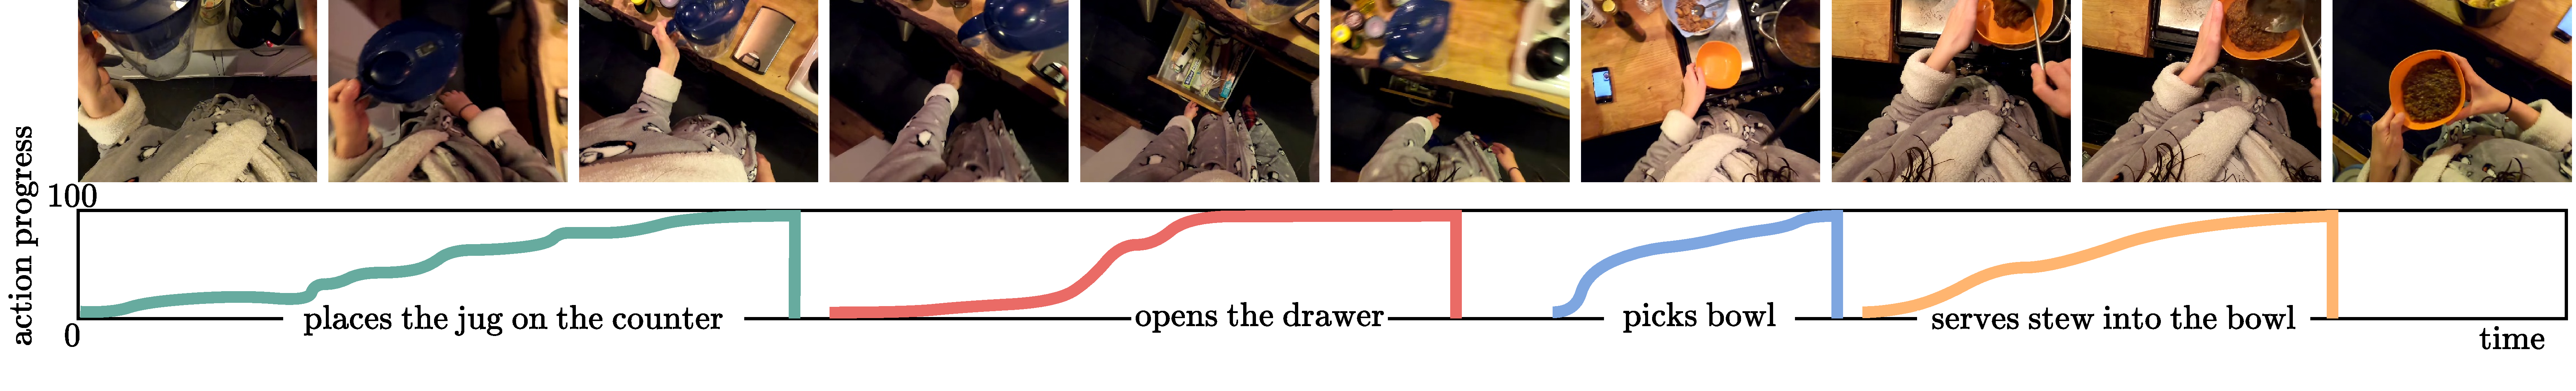
\includegraphics[width=\textwidth]{figs/states/states-action_progress.pdf}
\caption{\textbf{Action Process Prediction (APP)}. Given a video stream of a procedural task, estimate the progress of each ongoing action by inferring the time it will take to complete the action performed. Video sourced from \citet{grauman2024ego} \vspace{1em}}
\label{fig:states::progress}
\end{subfigure}
\begin{minipage}{0.49\textwidth}
\begin{subfigure}{\linewidth}
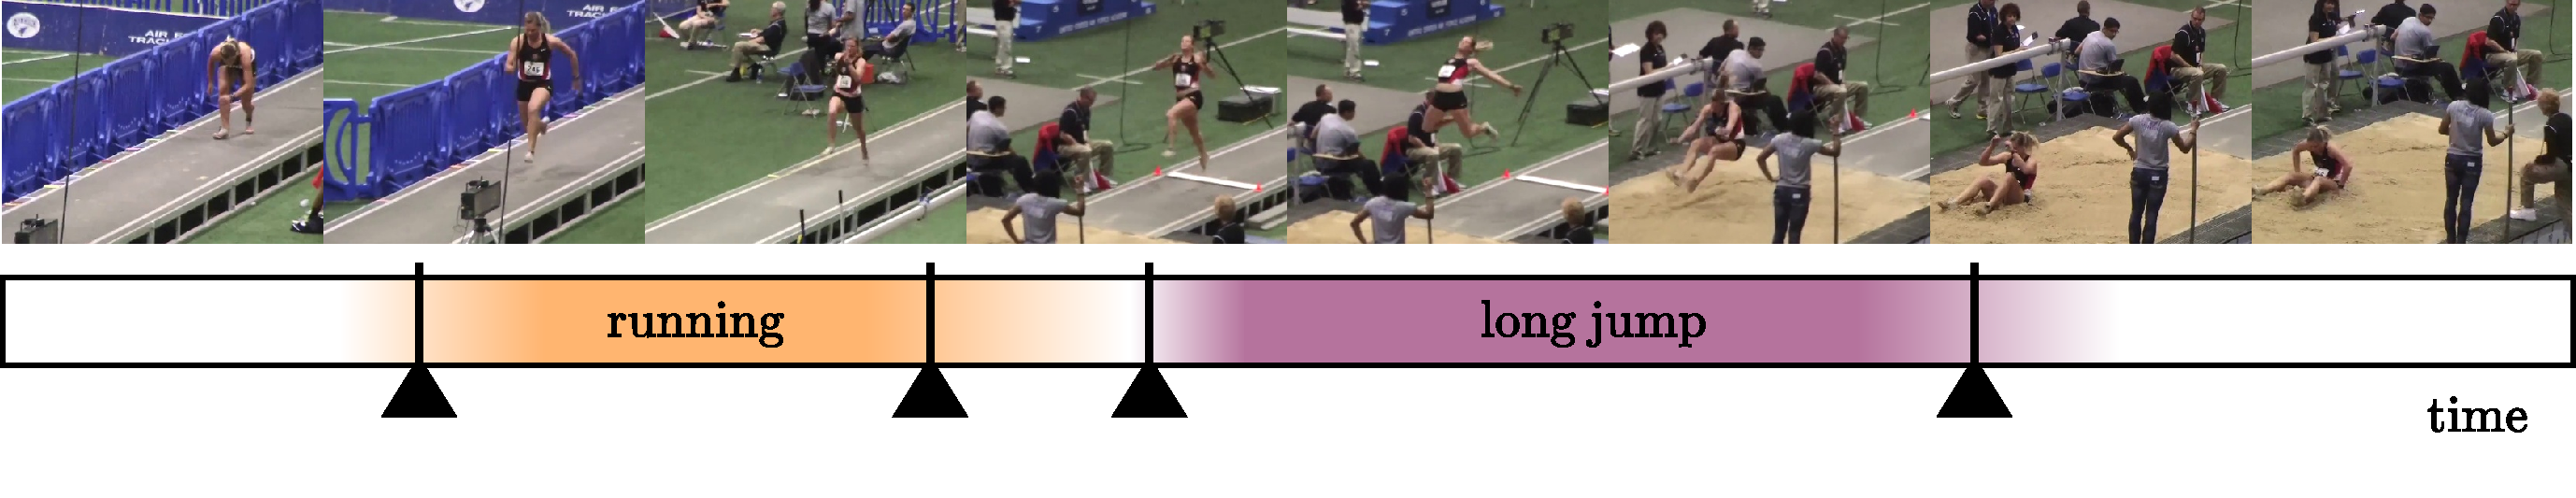
\includegraphics[width=\linewidth]{figs/states/states-event_boundary.pdf}
\caption{\textbf{Event Boundary Detection (EBD)}. Detect the start and end times of ongoing events in video streams. Video sourced from \citet{carreira2017quo} \vspace{1em}}
\label{fig:states::boundary}
\end{subfigure}
\hfill
\addtocounter{subfigure}{1}
\begin{subfigure}{\linewidth}
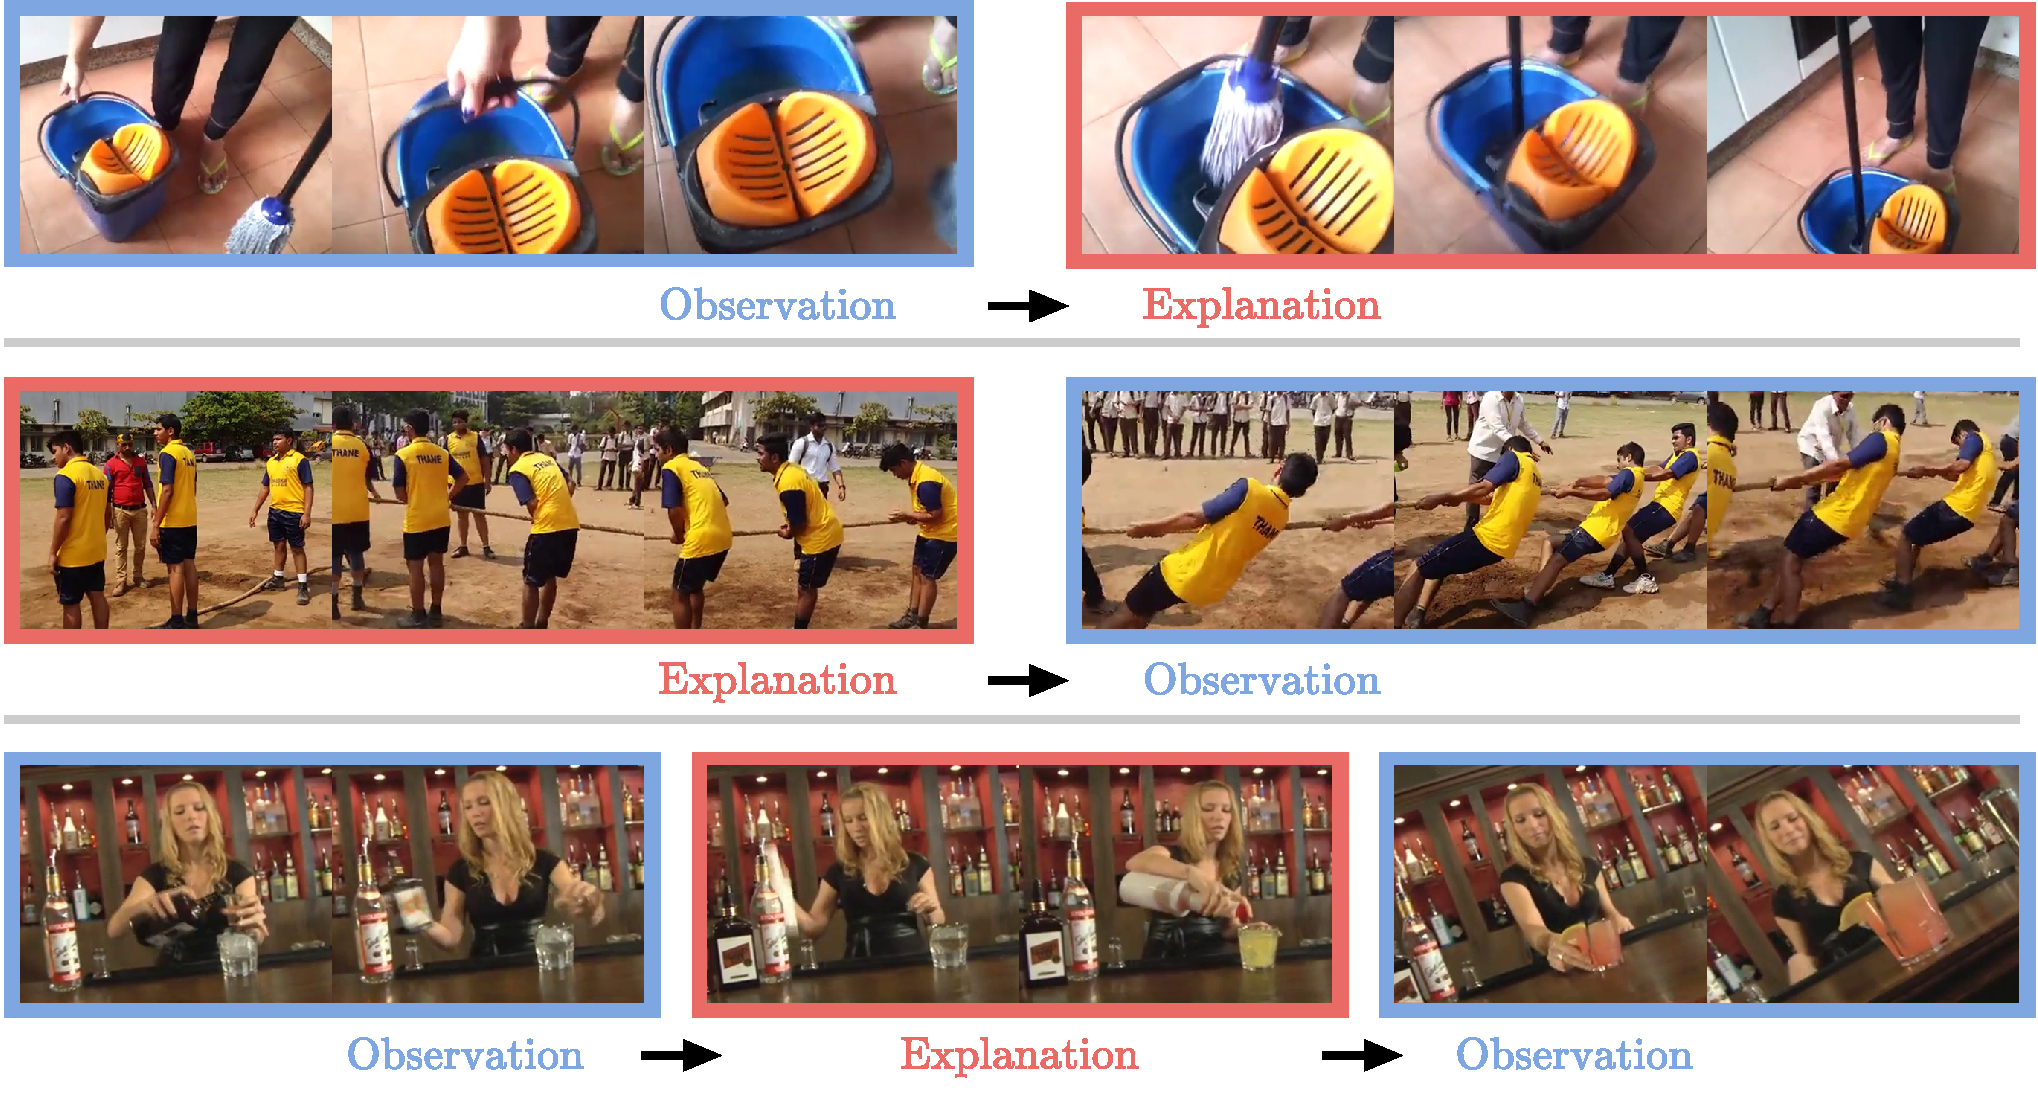
\includegraphics[width=\linewidth]{figs/states/states-abductive reasoning.pdf}
\caption{\textbf{Visual Abductive Reasoning (VAR)}. Given the observable part of the video in \textcolor{babyblue}{blue}, infer a likely explanation in \textcolor{fadedred}{red} for what follows before, after, or during the observation. The task requires a high-level understanding of the action or activity performed. Video sourced from \citet{liang2022visual} \vspace{1em}}
\label{fig:states::reasoning}
\end{subfigure}
\end{minipage}
\hfill
\begin{minipage}{0.49\textwidth} 
\addtocounter{subfigure}{-1} 
\begin{subfigure}{\linewidth}
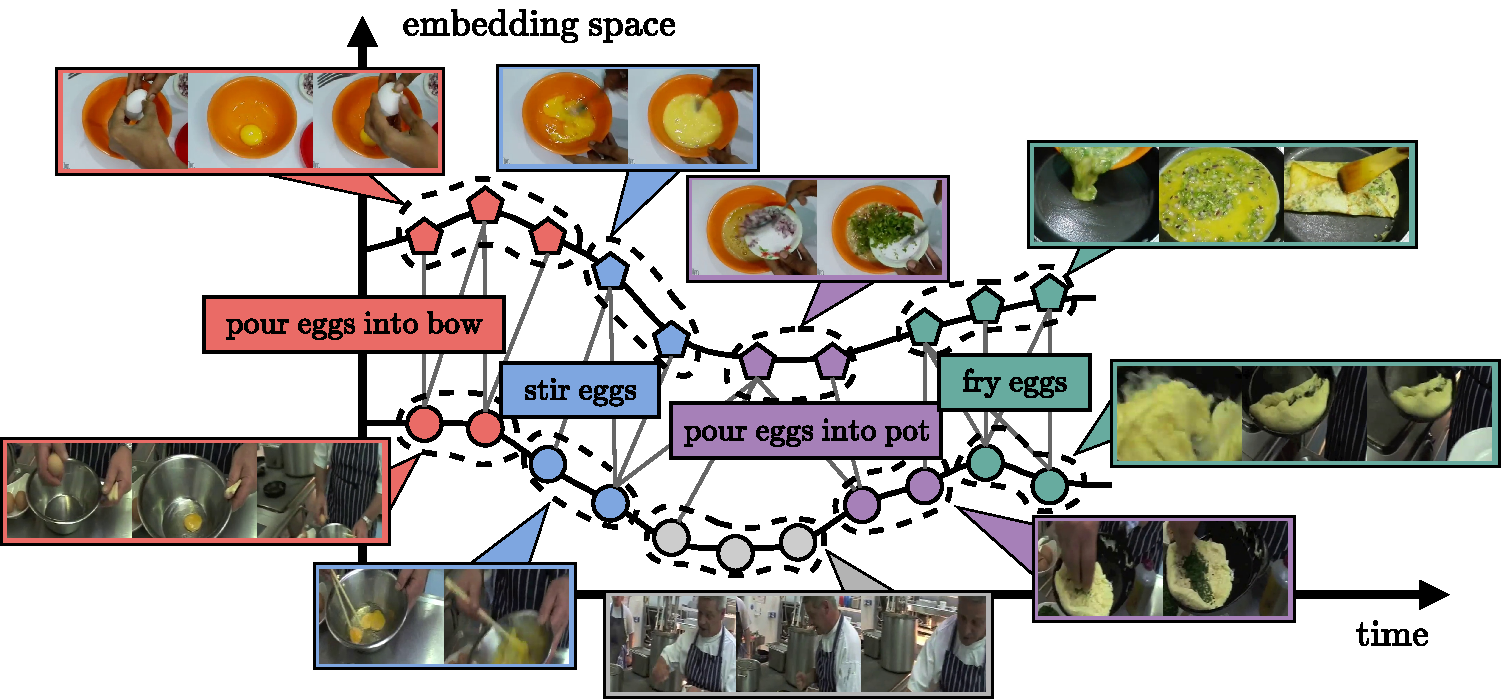
\includegraphics[width=\linewidth]{figs/states/states-alignment.pdf}
\caption{\textbf{Video Alignment (VA)}. Find correspondences across video instances with the same action performed and align them such that the execution of the action is synchronized. Video sourced from \citet{tang2019coin} \vspace{.5em}}
\label{fig:states::align}
\end{subfigure}
\hfill
\begin{subfigure}{\linewidth}
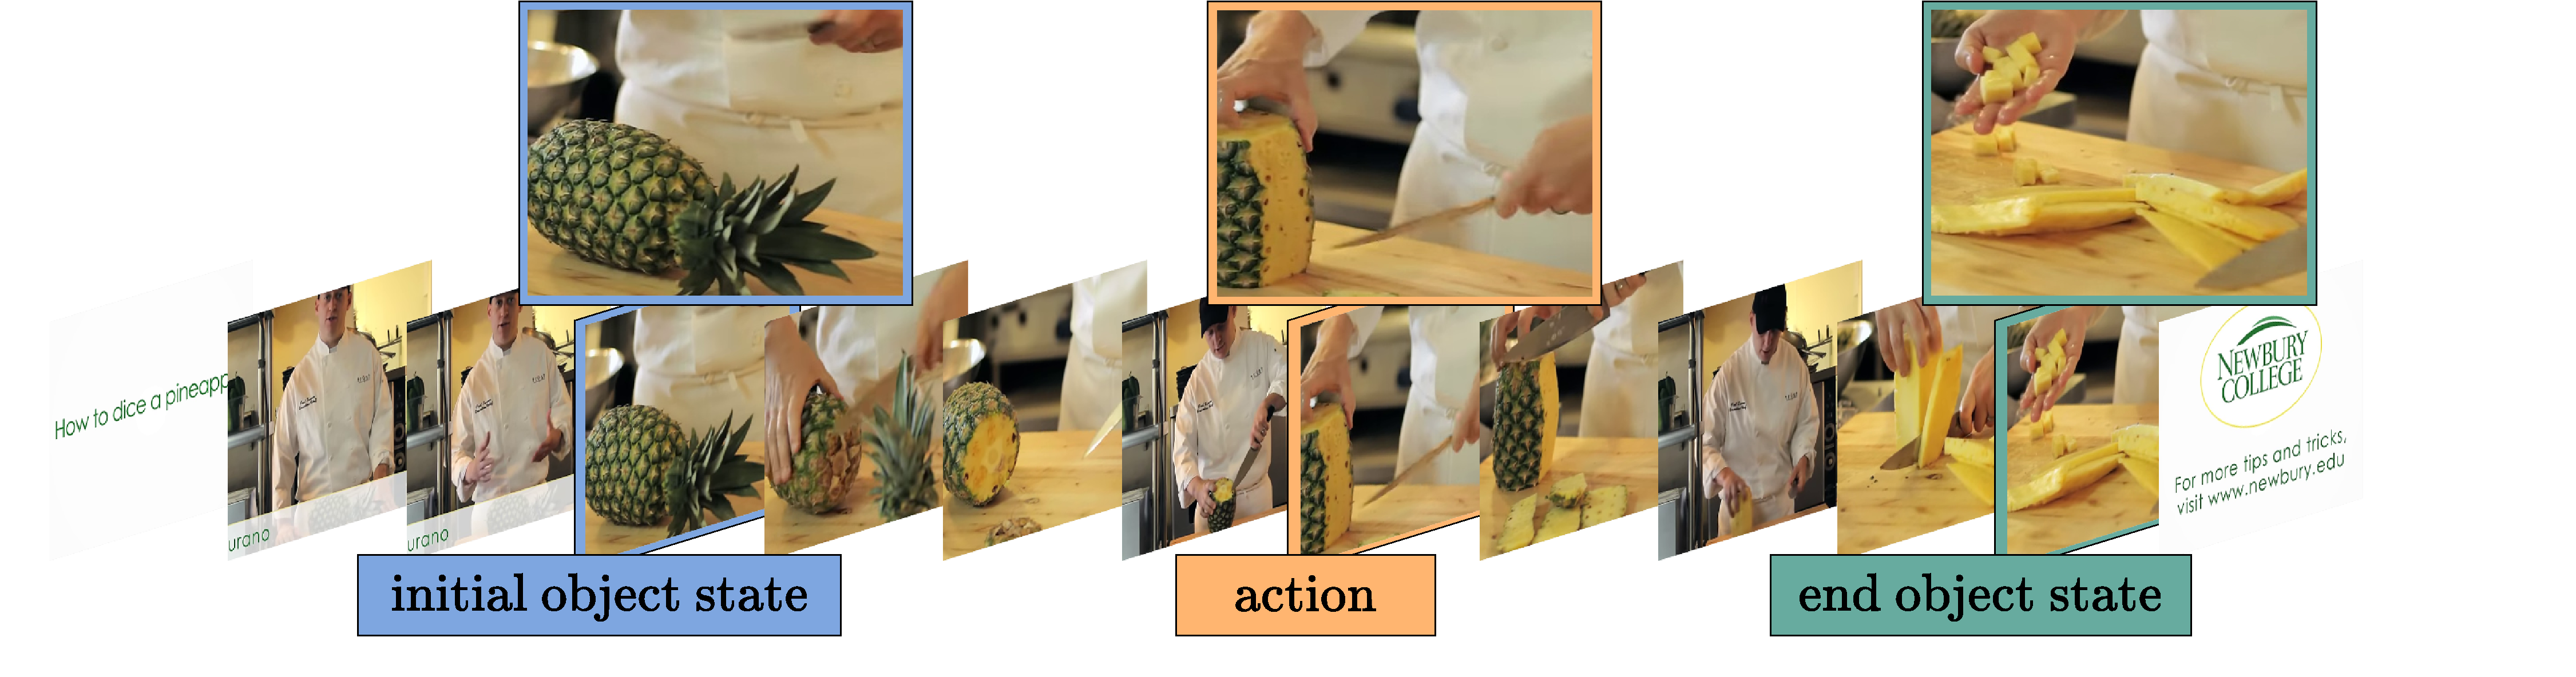
\includegraphics[width=\linewidth]{figs/states/states-object_state_change.pdf}
\caption{\textbf{Object State Change Detection (OSCD)}. State modifying actions such as \textit{cutting} progressively change the visual appearance of objects from an initial state in \textcolor{babyblue}{blue} to a final post-action execution state in \textcolor{pastelteal}{teal}. OSCD identifies the times that these changes occur. Video sourced from \citet{souvcek2022look}. \vspace{0.5em}}
\label{fig:states::oscd}
\end{subfigure}
\end{minipage} % end of second minipage
\begin{subfigure}{\linewidth}
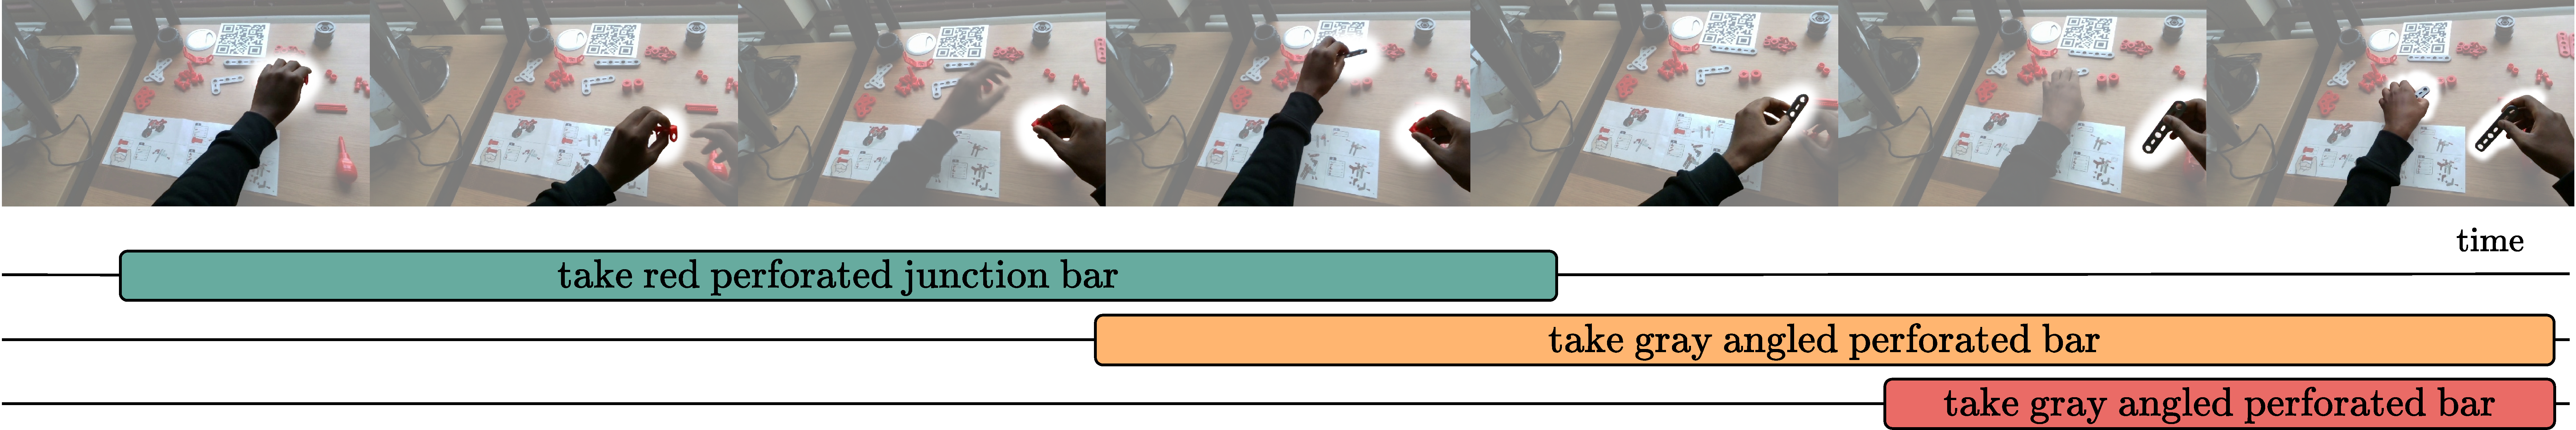
\includegraphics[width=\linewidth]{figs/states/states-active_object.pdf}
\caption{\textbf{Active Object Detection (AOD)}. Given a video in which a person interacts with multiple objects, AOD aims at detecting the object the person is currently using. Video sourced from \citep{ragusa2021meccano}.}
\label{fig:states::aod}
\end{subfigure}
\caption{\textbf{Tasks relating to object and action state change}. Each of the presented tasks can involve additional objectives.}
\label{fig:state_changes}
\end{figure*}



\subsection{State changes}
\label{sec:prediction::states}

Another set of action prediction tasks includes modeling the state changes in the environment, actions, objects, or execution speeds. Tracking, inferring, and reasoning in these tasks come with new sets of changes. An overview of the tasks' objectives is visualized in~\Cref{fig:state_changes}.

\subsubsection{Challenges}

Understanding the sequentially in videos is a central part of human perception. The translation of this to computer vision tasks remains challenging \citep{de2023there}. A central challenge relates to the \textbf{object state variability} as actions affect the visual appearance of objects in terms of shape, visibility, or perspective. Another set of challenges concerns actions with \textbf{non-rigid temporal boundaries}. Actions may not be easily distinguished from backgrounds or their execution may overlap with other actions. This presents \textbf{ambiguities in the action progress} as the completion of an action, or part of it, might also involve another action. Finally, the typically weak relation between visual input and the high-level semantic interpretation thereof complicates the training of robust, general models.



\subsubsection{State-based tasks}

We discuss six main tasks based on object and action state changes in their objectives.

% Progress
\noindent
\textbf{Action progress prediction (APP)}. Actions can be understood by procedural sets of motions performed towards an intended goal as shown in \Cref{fig:states::progress}. \citet{vaina1991object} suggested that understanding the state and progress of the action at different times can provide a holistic understanding of the intent and objective. In machine vision, an initial APP approach \citep{fathi2013modeling} used local descriptions to model per-frame state changes. \citep{kataoka2016recognition} used a descriptor to discover transitional actions within activity sequences. \citet{xiong2017pursuit} introduced a score function to distinguish between actions based on learned distinctive parts. \citet{becattini2020done} used actor and scene context information as an additional supervisory signal for APP. \citet{price2022unweavenet} expressed the progress of multiple actions through threads of activities that can overlap, a common situation in long procedural videos. \citet{shen2024progress} causally attended videos to define a task graph for APP over each action. More recently, generative approaches \citep{damen2024genhowto} using conditional control \citep{zhang2023adding} and procedural knowledge \citep{ashutosh2023video,zhou2023procedure} have been used to generate keyframes of changes. 

% Quality and completion
Another line of research works \citep{heidarivincheh2016beyond,heidarivincheh2018action} is aimed at localizing the moments that actions are completed. The speed of action completion or state changes in actions has also been studied in the context of skill determination \citep{doughty2018s} or their semantic correspondence to textual adverbs \citep{doughty2020action,doughty2022you,moltisanti2023learning}. Scoring approaches \citep{tang2020uncertainty} have been used to study the procedural execution of actions in the context of quality assessment. Adjacent tasks such as video captioning and action classification have also been integrated into multi-task settings \citep{parmar2019and}.


\noindent
\textbf{Event boundary detection (EBD)}. Different from the related well-studied task of action localization, EBD \citep{shou2021generic} aims at localizing event changes in videos \emph{regardless of the action classes}, shown in \Cref{fig:states::boundary}. \citet{aakur2019perceptual} proposed a self-supervised objective in which their model is initially trained to reconstruct subsequently observed features. \citep{shou2021generic} used a self-similarity metric to determine event boundaries by relating encoded frame features. Further, EBD approaches \citep{mounir2023streamer} have studied hierarchies of video events.

\noindent
\textbf{Video alignment (VA)}. As the performance of individual parts of actions can vary, video alignment, shown in \Cref{fig:states::align}, aims to temporally match key moments in the execution of the same action across videos. Initial efforts, motivated by temporal coherence \citep{goroshin2015unsupervised,fernando2017self,zhang2023modeling}, have studied VA based on Canonical Correlation Analysis (CCA) \citep{andrew2013deep} or by contrastively creating joint representations from multiple viewpoints \citep{sermanet2018time}. Dynamic Time Warping \citep{sakoe1978dynamic} is an algorithm that aligns variable length signals, and it has been adopted for VA \citep{chang2019d3tw,dvornik2021drop,hadji2021representation}. A more recent self-supervision objective \citep{dwibedi2018temporal} for VA is to train a video model to project per-frame embeddings in pairs of target videos by matching embeddings of one video to the nearest neighbor embeddings of the other. This approach was extended in subsequent works with the inclusion of context from the entire video \citep{haresh2021learning}, anchor frames to align redundant frames \citep{liu2022learning}, embeddings from text \citep{epstein2021learning}, and regularizers based on the correspondence to repetitions of the same action \citep{donahue2024learning}.


\noindent
\textbf{Visual abductive reasoning (VAR)}. A key element in action understanding is recovering the intended goal. High-level reasoning of events has initially been considered in hierarchies with rule-based approaches \citep{hakeem2004ontology} or the conditionality of action occurrences across different levels \citep{albanese2010pads}. \citet{pei2011parsing} detected atomic actions with graph representations to decompose complex events. VAR \citep{liang2022visual}, shown in \Cref{fig:states::reasoning}, is the vision-language task that uses characteristics of partial observations as a premise and requires formulating an explanation. Other VAR works have modeled intention by contrastively learning visual and language context \citep{li2023intentqa}, modeling timelines for news story understanding \citep{liu2023video}, and forecasting actions by multi-modal inputs \citep{zhu2023personality}. Evaluation of VAR models has also been studied in counterfactual vision-language pairs \citep{park2022exposing} similar to text-only tasks \citep{ippolito2019unsupervised,huang2020inset}.

\noindent
\textbf{Object state change detection (OSCD)}. Many actions alter the appearance or state of objects. OSCD approaches associate visual changes to changes in the states of objects in the scene, as shown in \Cref{fig:states::oscd}. Efforts \citep{alayrac2017joint,damen2014you,liu2017jointly,zhuo2019explainable} have initially focused on state modifications that do not involve significant appearance changes, \eg, `open/close door' or `fill/empty cup'. \citet{hong2021transformation} proposed a reasoning-based approach defining a triplet of complexities for single- and multi-step transformations with additional viewpoint changes. Other reasoning-based approaches include the use of language \citep{xue2024learning} and visual exemplars of start and end states \citep{souvcek2022look}. OSCD has also been studied in combination with other tasks including cross-state object segmentation \citep{yu2023video}, cross-action relevance \citep{alayrac2024multi}, or inspired by state-disentanglement for images \citep{gouidis2023leveraging,nagarajan2018attributes,saini2022disentangling}, generating start and end states by given context and scene prompts \citep{damen2024genhowto,saini2023chop}.

\noindent
\textbf{Active object detection (AOC)}. Actions can include multiple objects during their execution. Overviewed in \Cref{fig:states::aod}, AOD specifies the objects relevant to the currently performed atomic action. This task has recently gained interest as scenes can often be cluttered \citep{ragusa2021meccano} or a varying number of objects can be used for a single action \citep{miech2019howto100m}. \citet{nagarajan2019grounded} specifically focused on localizing the human-object interaction areas defining focal points of importance during the execution of actions. \citep{fu2021sequential} introduced a voting module over potential bounding boxes corresponding to the active object. \citet{kim2021hotr} used a parallelized model to detect instances and subsequently hand-object interactions. \citet{yang2024active} used scene context from text to define plausible interactions with target objects for AOD.  


\subsubsection{Future outlooks}

Similar to recent works in robotics that create goal-based policies \citep{kununi2024uni,wang2023manipulate}, state-understanding vision models require a holistic understanding of actions from a limited \textbf{availability of arbitrary object states}. Conceptually, the execution and changes in objects can be similar for different actions, \eg,\texttt{mixing a cake mix} and \texttt{whisking eggs}. Enforcing better learning objectives to improve this semantic correspondence can create more generalizable models with a better understanding of the physical world. In addition, the inclusion of cues from \textbf{supplementary modalities}, such as audio, can improve tasks that require relating parts of videos, as correspondences should be discoverable beyond the visual domain. This also presents the potential for creating general-purpose models based on \textbf{abductive reasoning} pre-text objectives that can then be applied to various downstream tasks.



\subsection{Anomaly detection}

Video Anomaly Detection (VAD) is the task of detecting unexpected actions or events in videos that deviate from predictable behaviors. Anomalies are detected through either explicitly classifying a pre-set number of actions in \textbf{close-set} settings or learning robust representations of the expected actions in \textbf{open-set} settings.


\subsubsection{Challenges}

VAD depends on strict binary annotations of normal and abnormal sequences, with most evaluation benchmarks including \textbf{limited definitions}. Even in the open-set settings, robust definitions are required for the target normal sequences. This prevents the creation of models that can estimate correctly unseen normal sequences. Another significant challenge for VAD models relates to their applicability. With their intended use in continuously operating surveillance systems, current approaches only \textbf{partially use temporal context} to infer predictions. Only a small number of approaches currently study the long-term effects of actions. Most datasets also only include modest temporal resolutions, limiting the exploration of context over longer time segments.



\subsubsection{Detecting anomalies in videos}

We identify two main approaches for the detection of anomalies in videos.

\noindent
\textbf{Close-set}. Anomalies can be discovered by \emph{close-set} tasks that aim to model both normal and abnormal sequences. \citet{sultani2018real} used Multiple Instance Ranking \citep{dietterich1997solving} to define positive groups that include videos with at least a single abnormal segment and negative groups of normal videos. The objective is to maximize the score between the assigned positive and negative groups. Subsequent efforts have built upon MIL with learned features \citep{dubey20193d}, or pseudo labels \citep{feng2021mist}. Approaches have also aimed to improve upon MIL's reliance on the dominant negative instances. \citet{zhang2019temporal} integrated inner-group sampling, \citet{pu2023learning,zhu2019motion} used temporal weighting, and \citet{tian2021weakly} maximized the separability between normal and anomalous representations. With a similar goal, the use of multiple temporal pretext tasks \citep{almarri2024multi,georgescu2021anomaly} and temporal scales \citep{li2022scale} have also been explored. \citet{chen2023mgfn} used a contrastive objective between representations of normal and abnormal videos. Clustering approaches focus on modeling sparsity \citep{lu2013abnormal}, enforcing high distribution variance in abnormalities \citep{li2021deep}, combining dense/spare clusters for normal/abnormal segments \citep{zaheer2020claws}, and using pseudo labels for anomalous segments \citep{zaheer2020self}. Another set of methods \citep{zhong2019graph,purwanto2021dance} has included graph networks to sequentially detect abnormal segments. More recent methods have distinguished between normal and anomalous states with the use of additional modalities such as audio \citep{wu2020not} and language context \citep{yang2024text,zanella2024harnessing}.


\begin{figure*}[!ht]
    \centering
    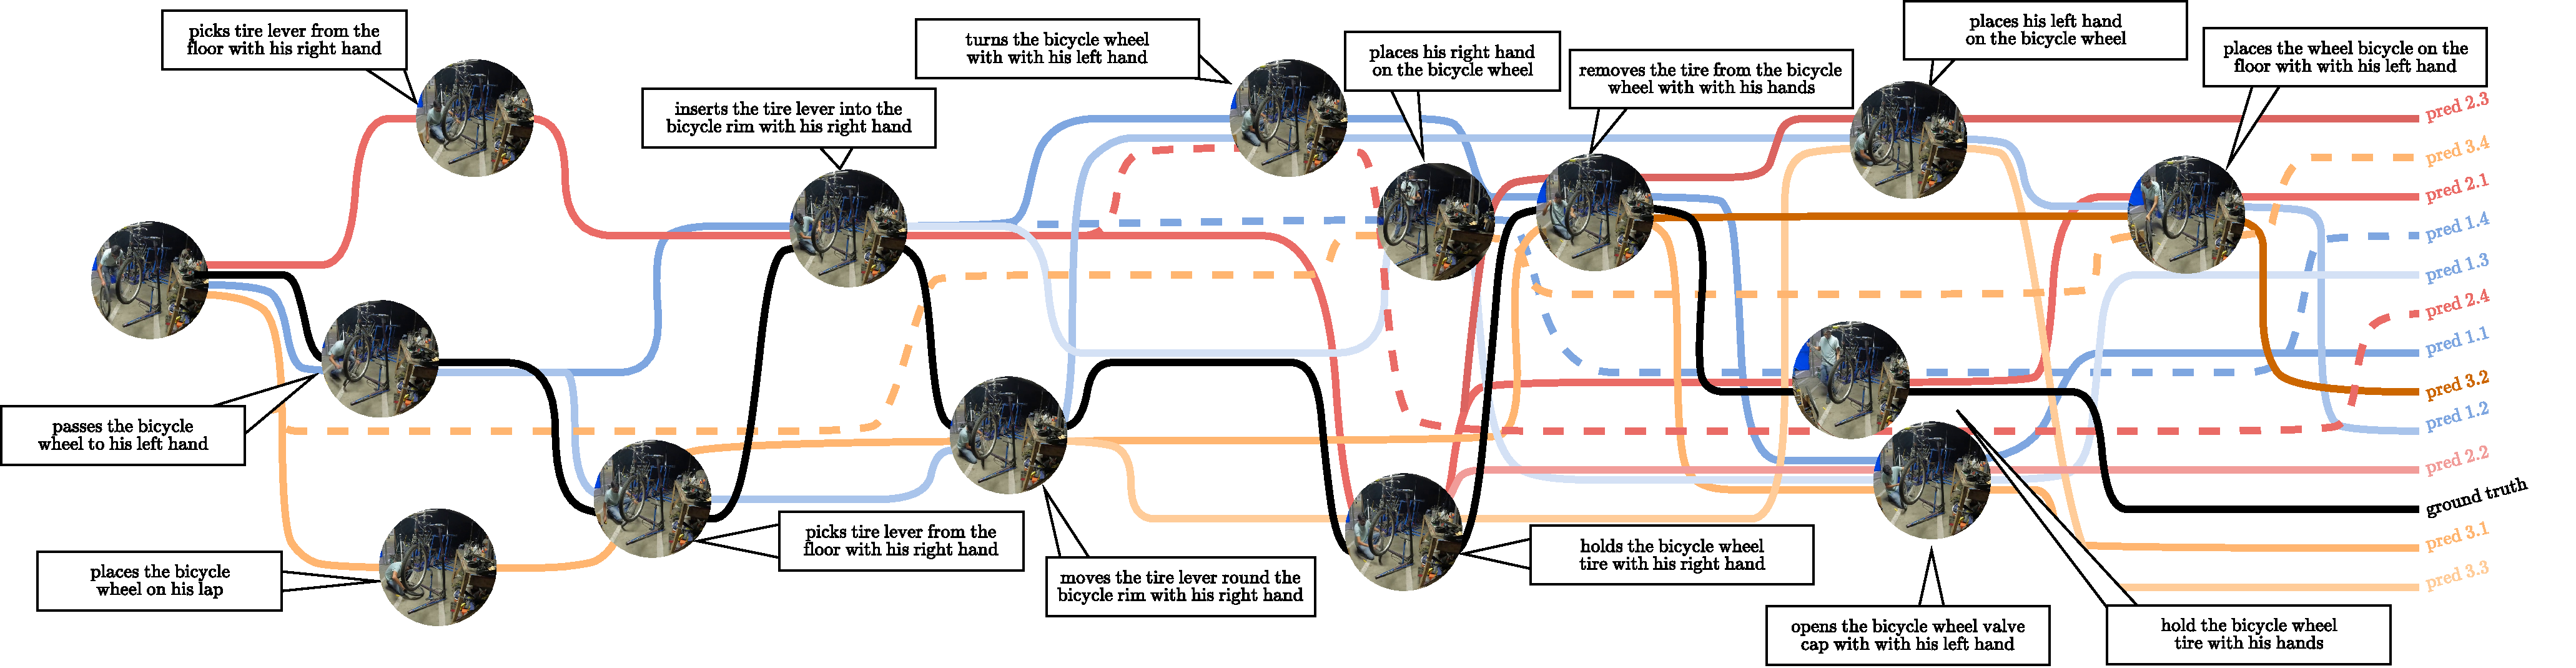
\includegraphics[width=\linewidth,trim={0cm 0 0cm 0},clip]{figs/narrative_chart_ego_exo.pdf}
    \caption{\textbf{Forecasting future actions}. Starting from the observed action, anticipation approaches infer the sequence of probable next actions. Predictions are shown in a narrative chart format similar to \citet{randal2009movie}.
    Example selected from \citet{grauman2024ego}.} 
    \label{fig:narration_chart}
\end{figure*}

\noindent
\textbf{Open-set}. As close-set solutions can only model abnormalities in labeled data, models cannot effectively generalize to distributions different than those seen during training. This issue has been studied by \citet{zhao2011online} and \citet{luo2017revisit} as a sparse-coding \citep{lee2006efficient} problem in which the model is trained to reconstruct normal sequences. Abnormalities can then be inferred through the reconstruction loss. Temporal regularity can also be modeled with autoencoders as a reconstruction task \citep{hasan2016learning}. To deal with the scarcity of abnormal sequences during training, autoencoder (AE)-based approaches use pseudo representations to improve the embedding space \citep{astrid2021synthetic,astrid2021learning}. \citet{park2020learning} learned prototypes of normal sequences which can then be used to contrast query videos. Other works have constrained the representation space of normal sequences by optimizing piecewise linear decision boundaries \citep{wang2019gods}. Two-steam AE frameworks \citep{cho2022unsupervised,nguyen2019anomaly} have been used to separately reconstruct the appearance and motion characteristics of normal sequences. Generative approaches \citep{micorek2024mulde} have recently focused on the latent space with Gaussian Mixture Model (GMM) and inferred an anomaly score across all noise levels. \citet{fioresi2023ted} has also explored cross-frame mutual information minimization in tandem with a generative objective for privacy preservation. Other privacy-aimed approaches have studied trajectory-based video anomaly detection. \citet{morais2019learning} used an RNN to track skeletal points and regressed future locations. The objective of the model was to learn a fixed interpolation for normal sequences with abnormalities captured by the large reconstruction error. Subsequent approaches have used a similar objective to train graph networks \citep{markovitz2020graph}, probabilistic models \citep{flaborea2023multimodal}, and masked autoencoders \citep{stergiou2024holistic}.


\subsubsection{Future outlooks}

Although great progress has been made, most VAD methods still require adjusting the definitions of normal sequences to update predictions. A direction for future works can be a unified framework that can efficiently adapt predictions through \textbf{life-long learning}. Recent works \citep{yang2024text,zanella2024harnessing} fused frame-wise language descriptions from LLMs without requirements for re-training the visual model which can be an effective strategy for novel scene VAD. However, these approaches are based on the accuracy of the produced summaries with video-language misalignment directly impacting performance. Potential improvements may explore \textbf{in-context learning}. \citet{zhao2024can} showed that progressively increasing task difficulty through prompts can aid the generalization ability of models to unseen visual scenes.
